\chapter{Insights}

\section{Typical Words}

\subsection{Tf-Idf}
How did we define typical words for tf-idf:
\begin{itemize}
	\item define tf-idf genre vectors by averaging all document vectors of given genre (on training set)
	\item compute an average tf-idf vector of the whole training set
	\item subtract the average vector from each genre vector
	\item The most important words are those with highest scores
	\item Based on desired output, filter out too short words (having only two characters) and rare words (e.g. keep only those which occurred at least in $0.5\ \%$ of documents)
	\item investigate words with highest and lowest variance in tf-idf coefficient among the $14$ genre vectors
\end{itemize}

\subsection{Doc2Vec}
\begin{itemize}
	\item look at words most similar to the trained genre vectors
\end{itemize}

As we trained also word embeddings for the doc2vec model, we can look at similarities between a document and a word. To get a representative vector of a given genre, we average all vectors of that genre. 

Next, we compute dot products between the genre vector and all words in the vocabulary. As we want to get representative words of the genre, we filter out uncommon words which occured in less than $0.5\ \%$ of all documents. We also focus only on words consisting of at least 4 letters, as shorter words seem to have higher similarity to all documents in general when computed based on dot product. \cref{fig:typical_words_genre} shows a word cloud of most typical words for \textit{detective and mystery stories}, \textit{science fiction} and \textit{western stories}.


When using different similarity metrics, the typical words didn't seem too meaningful. For \textit{cosine similarity}, due to normalization, shorter words tend to be much more similar to all documents in general than other words. For euclidean metric, All genres gave same typical words.


\section{Document similarity}
Choose a document and find most similar documents. Look at accuracy @ 1, 3, 5, 10 documents for the following:
\begin{itemize}
	\item Are they part of the same book? - 
	\item Same author?
	\item Same genre?
\end{itemize}


\begin{figure}[h]
	\centering
	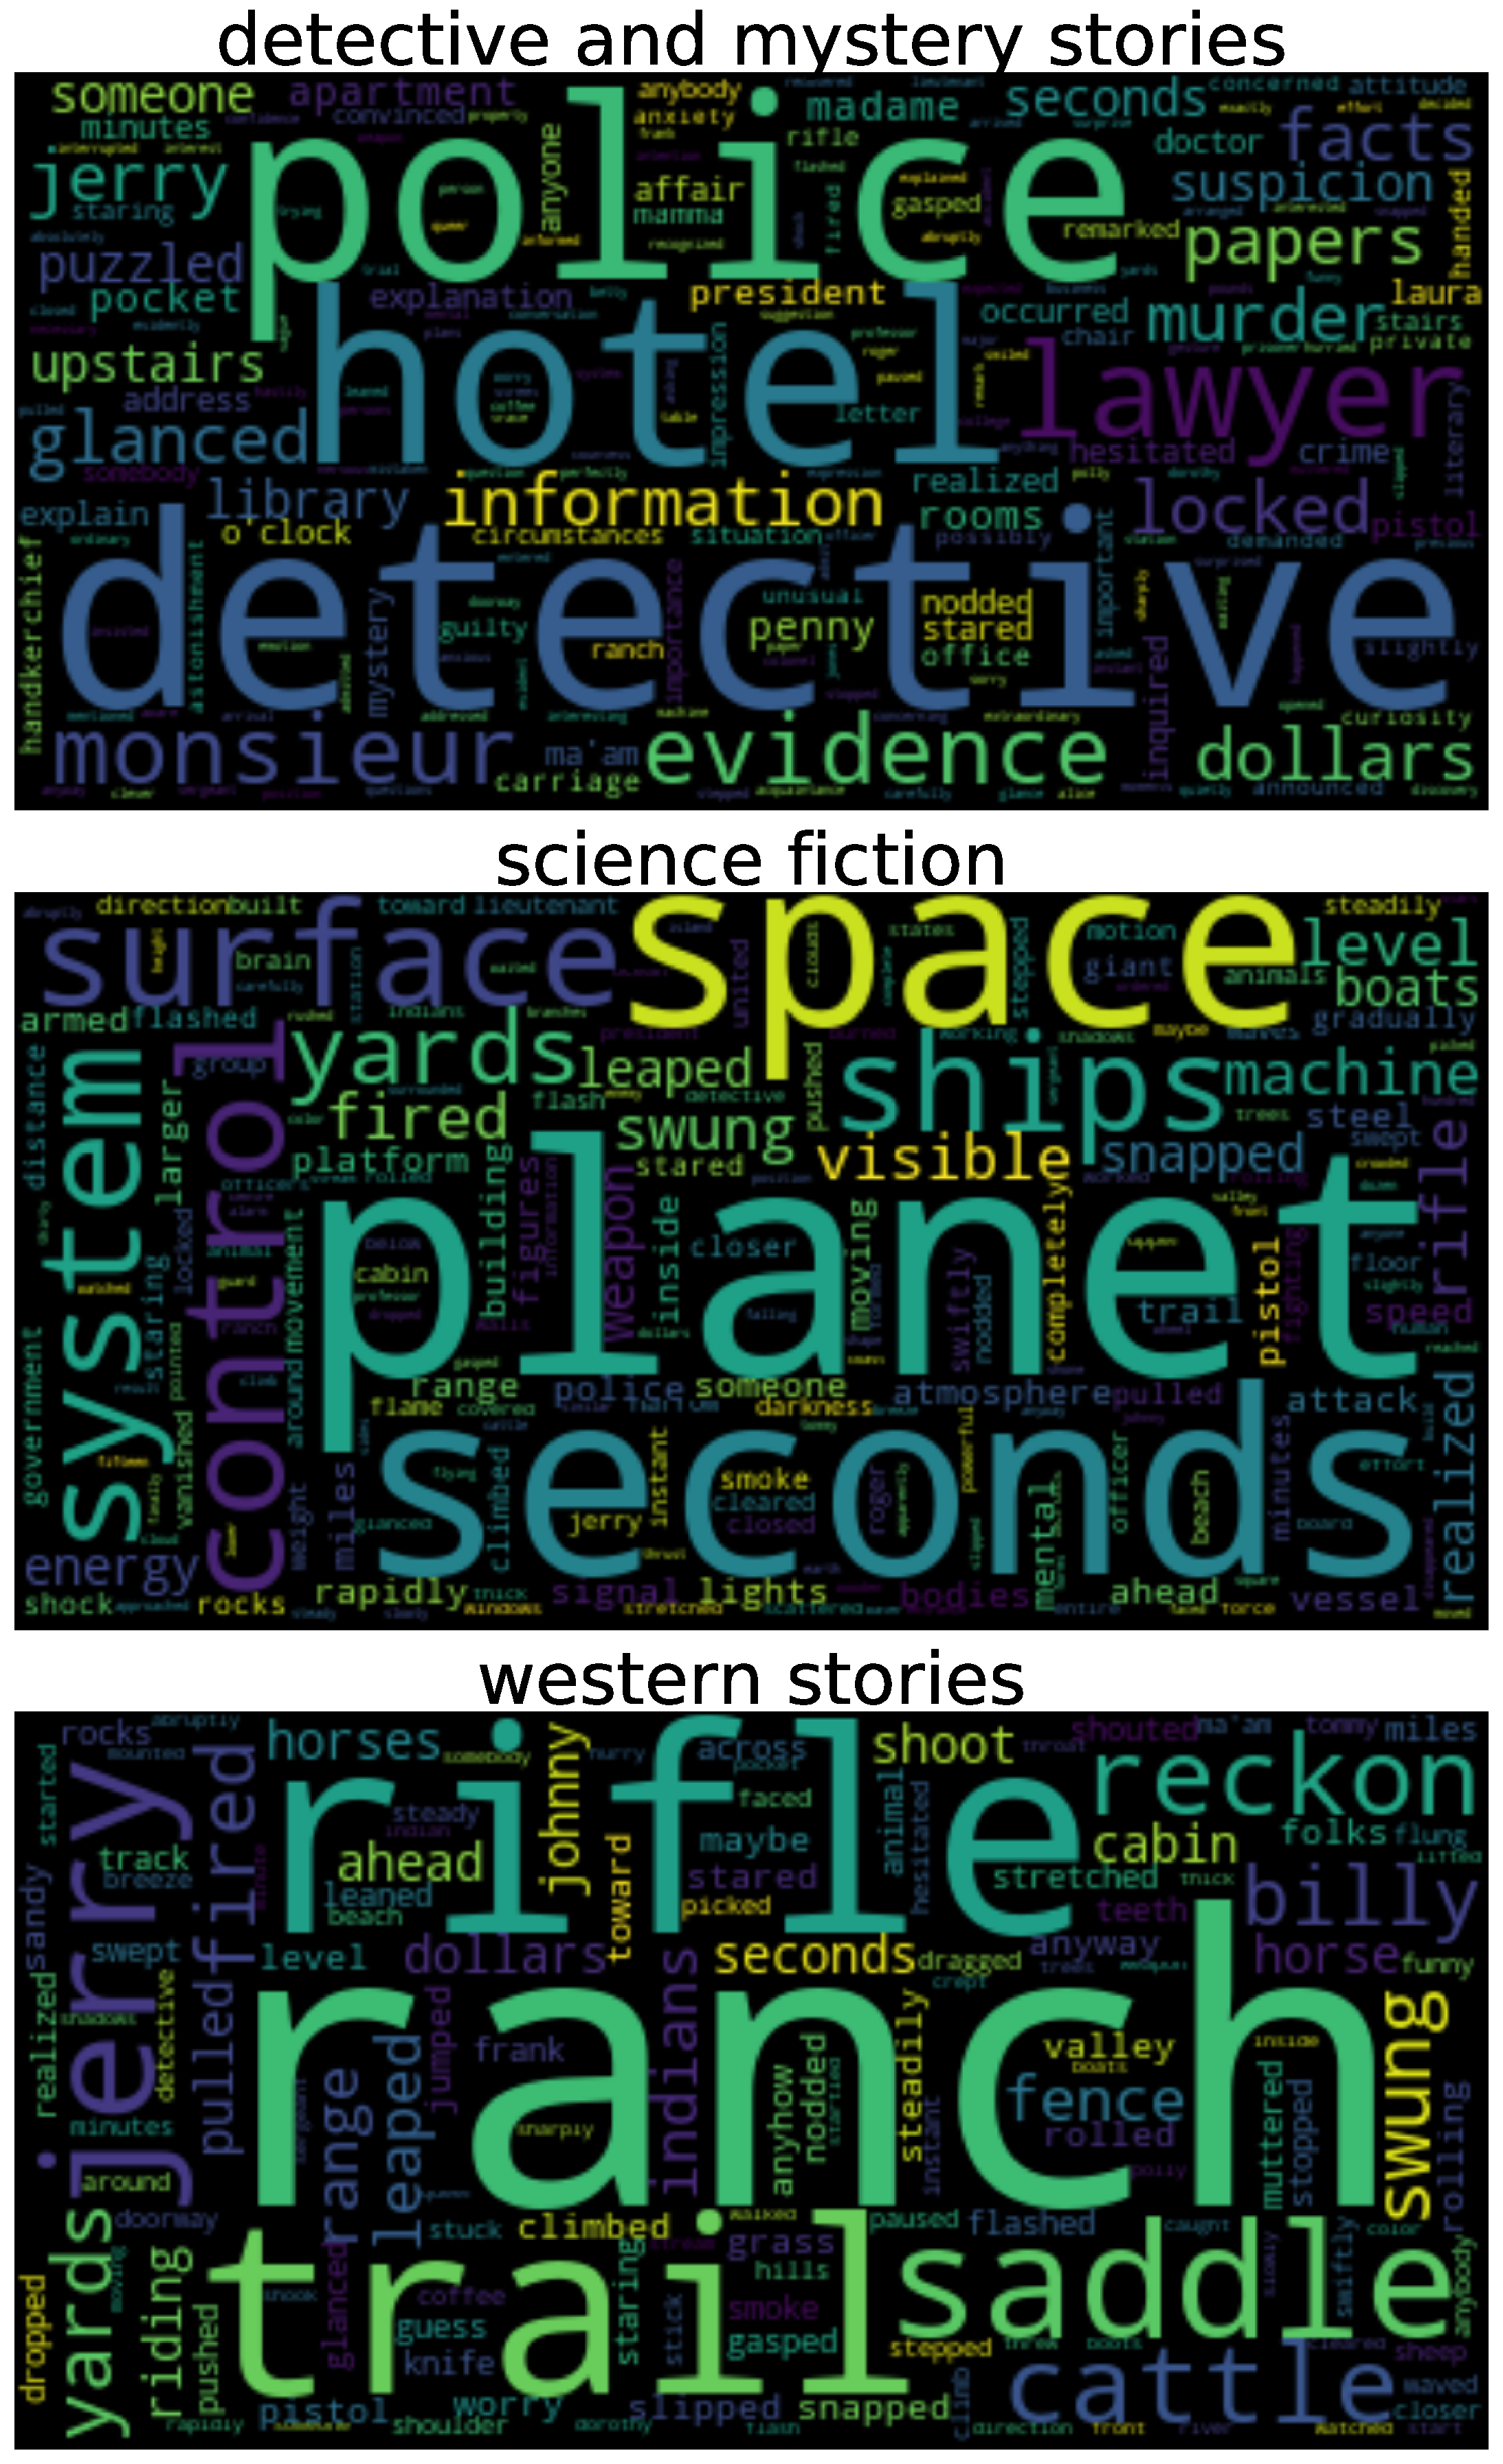
\includegraphics[height=0.6\textheight]{img/06_typical_words_genre}
	\caption{Typical words for \textit{detective and mystery stories}, \textit{science fiction} and \textit{western stories} based on doc2vec and dot product document-word similarity.}
	\label{fig:typical_words_genre}
\end{figure}

\section{Visualizing document vectors}
To visualize documents in 2D, we transformed the document vectors to $2$ dimensions using dimensionality reduction techniques. The final plot is made by t-SNE algorithm. However, as the convergence takes very long for large datasets, we first run PCA and transformed the data to $50$ dimensions and run t-SNE on those.
